% Options for packages loaded elsewhere
\PassOptionsToPackage{unicode}{hyperref}
\PassOptionsToPackage{hyphens}{url}
\PassOptionsToPackage{dvipsnames,svgnames,x11names}{xcolor}
%
\documentclass[
  letterpaper,
  DIV=11,
  numbers=noendperiod]{scrartcl}

\usepackage{amsmath,amssymb}
\usepackage{lmodern}
\usepackage{iftex}
\ifPDFTeX
  \usepackage[T1]{fontenc}
  \usepackage[utf8]{inputenc}
  \usepackage{textcomp} % provide euro and other symbols
\else % if luatex or xetex
  \usepackage{unicode-math}
  \defaultfontfeatures{Scale=MatchLowercase}
  \defaultfontfeatures[\rmfamily]{Ligatures=TeX,Scale=1}
\fi
% Use upquote if available, for straight quotes in verbatim environments
\IfFileExists{upquote.sty}{\usepackage{upquote}}{}
\IfFileExists{microtype.sty}{% use microtype if available
  \usepackage[]{microtype}
  \UseMicrotypeSet[protrusion]{basicmath} % disable protrusion for tt fonts
}{}
\makeatletter
\@ifundefined{KOMAClassName}{% if non-KOMA class
  \IfFileExists{parskip.sty}{%
    \usepackage{parskip}
  }{% else
    \setlength{\parindent}{0pt}
    \setlength{\parskip}{6pt plus 2pt minus 1pt}}
}{% if KOMA class
  \KOMAoptions{parskip=half}}
\makeatother
\usepackage{xcolor}
\setlength{\emergencystretch}{3em} % prevent overfull lines
\setcounter{secnumdepth}{-\maxdimen} % remove section numbering
% Make \paragraph and \subparagraph free-standing
\ifx\paragraph\undefined\else
  \let\oldparagraph\paragraph
  \renewcommand{\paragraph}[1]{\oldparagraph{#1}\mbox{}}
\fi
\ifx\subparagraph\undefined\else
  \let\oldsubparagraph\subparagraph
  \renewcommand{\subparagraph}[1]{\oldsubparagraph{#1}\mbox{}}
\fi


\providecommand{\tightlist}{%
  \setlength{\itemsep}{0pt}\setlength{\parskip}{0pt}}\usepackage{longtable,booktabs,array}
\usepackage{calc} % for calculating minipage widths
% Correct order of tables after \paragraph or \subparagraph
\usepackage{etoolbox}
\makeatletter
\patchcmd\longtable{\par}{\if@noskipsec\mbox{}\fi\par}{}{}
\makeatother
% Allow footnotes in longtable head/foot
\IfFileExists{footnotehyper.sty}{\usepackage{footnotehyper}}{\usepackage{footnote}}
\makesavenoteenv{longtable}
\usepackage{graphicx}
\makeatletter
\def\maxwidth{\ifdim\Gin@nat@width>\linewidth\linewidth\else\Gin@nat@width\fi}
\def\maxheight{\ifdim\Gin@nat@height>\textheight\textheight\else\Gin@nat@height\fi}
\makeatother
% Scale images if necessary, so that they will not overflow the page
% margins by default, and it is still possible to overwrite the defaults
% using explicit options in \includegraphics[width, height, ...]{}
\setkeys{Gin}{width=\maxwidth,height=\maxheight,keepaspectratio}
% Set default figure placement to htbp
\makeatletter
\def\fps@figure{htbp}
\makeatother

\usepackage{booktabs}
\usepackage{longtable}
\usepackage{array}
\usepackage{multirow}
\usepackage{wrapfig}
\usepackage{float}
\usepackage{colortbl}
\usepackage{pdflscape}
\usepackage{tabu}
\usepackage{threeparttable}
\usepackage{threeparttablex}
\usepackage[normalem]{ulem}
\usepackage{makecell}
\usepackage{xcolor}
\usepackage{caption}
\usepackage{graphicx}
\usepackage{siunitx}
\usepackage{hhline}
\usepackage{calc}
\usepackage{tabularx}
\usepackage{adjustbox}
\usepackage{hyperref}
\KOMAoption{captions}{tableheading}
\makeatletter
\makeatother
\makeatletter
\makeatother
\makeatletter
\@ifpackageloaded{caption}{}{\usepackage{caption}}
\AtBeginDocument{%
\ifdefined\contentsname
  \renewcommand*\contentsname{Table of contents}
\else
  \newcommand\contentsname{Table of contents}
\fi
\ifdefined\listfigurename
  \renewcommand*\listfigurename{List of Figures}
\else
  \newcommand\listfigurename{List of Figures}
\fi
\ifdefined\listtablename
  \renewcommand*\listtablename{List of Tables}
\else
  \newcommand\listtablename{List of Tables}
\fi
\ifdefined\figurename
  \renewcommand*\figurename{Figure}
\else
  \newcommand\figurename{Figure}
\fi
\ifdefined\tablename
  \renewcommand*\tablename{Table}
\else
  \newcommand\tablename{Table}
\fi
}
\@ifpackageloaded{float}{}{\usepackage{float}}
\floatstyle{ruled}
\@ifundefined{c@chapter}{\newfloat{codelisting}{h}{lop}}{\newfloat{codelisting}{h}{lop}[chapter]}
\floatname{codelisting}{Listing}
\newcommand*\listoflistings{\listof{codelisting}{List of Listings}}
\makeatother
\makeatletter
\@ifpackageloaded{caption}{}{\usepackage{caption}}
\@ifpackageloaded{subcaption}{}{\usepackage{subcaption}}
\makeatother
\makeatletter
\@ifpackageloaded{tcolorbox}{}{\usepackage[many]{tcolorbox}}
\makeatother
\makeatletter
\@ifundefined{shadecolor}{\definecolor{shadecolor}{rgb}{.97, .97, .97}}
\makeatother
\makeatletter
\makeatother
\ifLuaTeX
  \usepackage{selnolig}  % disable illegal ligatures
\fi
\IfFileExists{bookmark.sty}{\usepackage{bookmark}}{\usepackage{hyperref}}
\IfFileExists{xurl.sty}{\usepackage{xurl}}{} % add URL line breaks if available
\urlstyle{same} % disable monospaced font for URLs
\hypersetup{
  pdftitle={Spurious Regressions Asad Zaman },
  pdfauthor={Zahid Asghar },
  colorlinks=true,
  linkcolor={blue},
  filecolor={Maroon},
  citecolor={Blue},
  urlcolor={Blue},
  pdfcreator={LaTeX via pandoc}}

\title{\textbf{\href{https://weapedagogy.wordpress.com/2021/04/30/spurious-regressions/}{Spurious
Regressions Asad Zaman} }}
\usepackage{etoolbox}
\makeatletter
\providecommand{\subtitle}[1]{% add subtitle to \maketitle
  \apptocmd{\@title}{\par {\large #1 \par}}{}{}
}
\makeatother
\subtitle{Reproduced in Quarto in R by the Author}
\author{\emph{Zahid Asghar }}
\date{12/13/22}

\begin{document}
\maketitle
\ifdefined\Shaded\renewenvironment{Shaded}{\begin{tcolorbox}[borderline west={3pt}{0pt}{shadecolor}, frame hidden, breakable, boxrule=0pt, enhanced, interior hidden, sharp corners]}{\end{tcolorbox}}\fi

\renewcommand*\contentsname{Table of contents}
{
\hypersetup{linkcolor=}
\setcounter{tocdepth}{3}
\tableofcontents
}
\hypertarget{introduction}{%
\subsection{Introduction}\label{introduction}}

In previous lectures
\href{https://weapedagogy.wordpress.com/2021/04/19/causal-explanation-of-autonomy-invariance-of-regression-relationships/}{Causal
Explanation of Autonomy \& Invariance of Regression Relationships}, we
have seen the essential importance of analyzing the causal structure of
the variables under study via path diagrams. In this lecture, we study
one aspect of this which creates serious problems for understanding and
interpreting regression results. This is the problem of a common cause.

\(Z\) is a common cause of \(X\) and \(Y\) if \(Z\) \(\Rightarrow\)
\(X\) and \(Z\) \(\Rightarrow\) \(Y\). When this happens, \(X\) and
\(Y\) will be correlated, but neither variable causes the other. In such
situations, a regression of \(Y\) on \(X\) will give results which show,
according to standard methods for analysis, that \(X\) is a strong
determinant of \(Y\). This is called a \emph{spurious} regression, or a
\emph{nonsense} regression. In this lecture, we will study some examples
of this phenomena in real world data.

\hypertarget{a-causal-relationship-a-consumption-function}{%
\subsection{A Causal Relationship: A Consumption
Function}\label{a-causal-relationship-a-consumption-function}}

Data on annual GDP, Consumption, and Investment, for Singapore, taken
from the WDI data set of the World Bank, is plotted below:

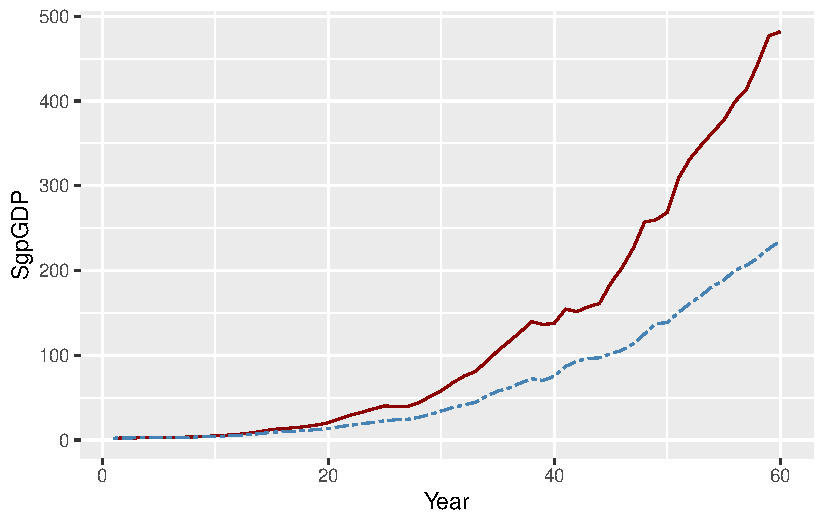
\includegraphics{Spurious-Regressions_files/figure-pdf/unnamed-chunk-1-1.pdf}

The Keynesian consumption function is one of the most widely accepted
and estimated regression models. The causal hypothesis is that Income
(GDP) determines Consumption (Con): GDP \(Rightarrow\) Con. The simplest
regression model which embodies this relationship is: Con = a + b GDP.
Running this regression on the data leads to the following results:

\begin{verbatim}
# A tibble: 60 x 5
      ID SgpCon SgpGDP SgpCon_hat residual
   <int>  <dbl>  <dbl>      <dbl>    <dbl>
 1     1   2.09   2.04       5.42    -3.33
 2     2   2.33   2.22       5.51    -3.18
 3     3   2.44   2.40       5.60    -3.15
 4     4   2.61   2.68       5.73    -3.12
 5     5   2.53   2.60       5.69    -3.16
 6     6   2.66   2.82       5.80    -3.13
 7     7   2.92   3.17       5.97    -3.04
 8     8   3.25   3.60       6.18    -2.92
 9     9   3.65   4.15       6.44    -2.79
10    10   4.02   4.82       6.77    -2.74
# ... with 50 more rows
\end{verbatim}

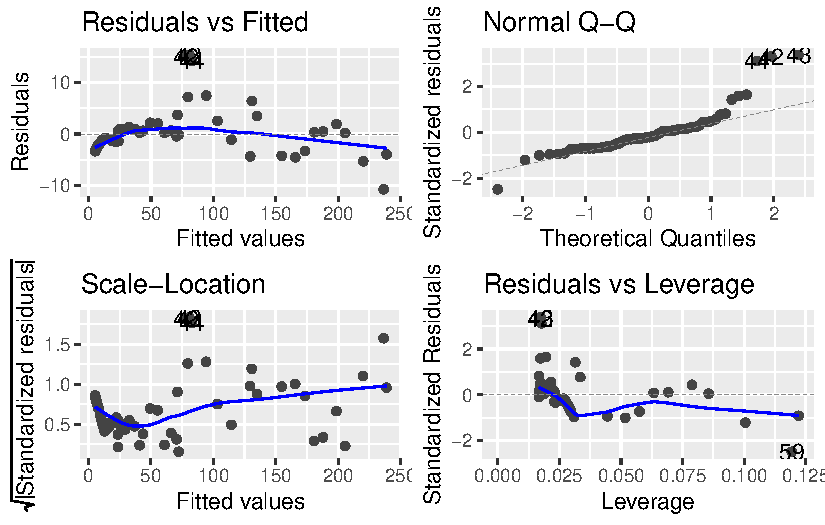
\includegraphics{Spurious-Regressions_files/figure-pdf/unnamed-chunk-2-1.pdf}

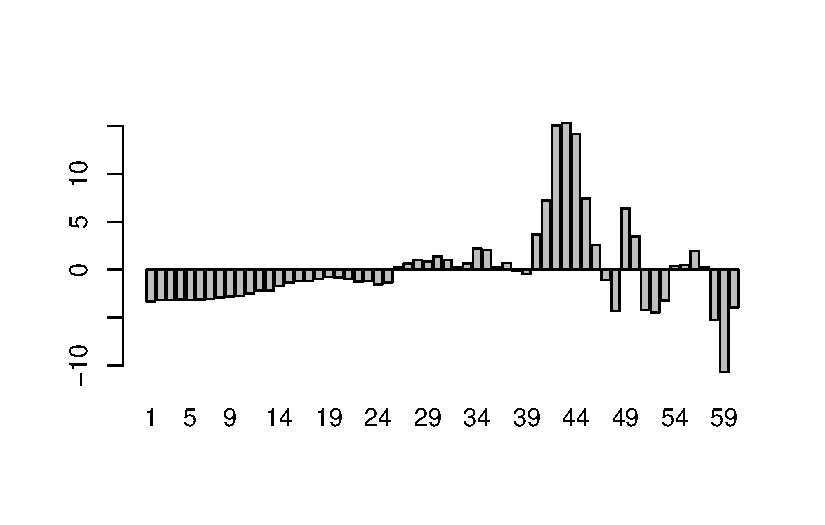
\includegraphics{Spurious-Regressions_files/figure-pdf/unnamed-chunk-2-2.pdf}

 
  \providecommand{\huxb}[2]{\arrayrulecolor[RGB]{#1}\global\arrayrulewidth=#2pt}
  \providecommand{\huxvb}[2]{\color[RGB]{#1}\vrule width #2pt}
  \providecommand{\huxtpad}[1]{\rule{0pt}{#1}}
  \providecommand{\huxbpad}[1]{\rule[-#1]{0pt}{#1}}

\begin{table}[ht]
\begin{centerbox}
\begin{threeparttable}
 
\setlength{\tabcolsep}{0pt}
\begin{tabular}{l l}


\hhline{>{\huxb{0, 0, 0}{0.8}}->{\huxb{0, 0, 0}{0.8}}-}
\arrayrulecolor{black}

\multicolumn{1}{!{\huxvb{0, 0, 0}{0}}c!{\huxvb{0, 0, 0}{0}}}{\huxtpad{6pt + 1em}\centering \hspace{6pt}  \hspace{6pt}\huxbpad{6pt}} &
\multicolumn{1}{c!{\huxvb{0, 0, 0}{0}}}{\huxtpad{6pt + 1em}\centering \hspace{6pt} (1) \hspace{6pt}\huxbpad{6pt}} \tabularnewline[-0.5pt]


\hhline{>{\huxb{255, 255, 255}{0.4}}->{\huxb{0, 0, 0}{0.4}}-}
\arrayrulecolor{black}

\multicolumn{1}{!{\huxvb{0, 0, 0}{0}}l!{\huxvb{0, 0, 0}{0}}}{\huxtpad{6pt + 1em}\raggedright \hspace{6pt} (Intercept) \hspace{6pt}\huxbpad{6pt}} &
\multicolumn{1}{r!{\huxvb{0, 0, 0}{0}}}{\huxtpad{6pt + 1em}\raggedleft \hspace{6pt} 4.425 *** \hspace{6pt}\huxbpad{6pt}} \tabularnewline[-0.5pt]


\hhline{}
\arrayrulecolor{black}

\multicolumn{1}{!{\huxvb{0, 0, 0}{0}}l!{\huxvb{0, 0, 0}{0}}}{\huxtpad{6pt + 1em}\raggedright \hspace{6pt}  \hspace{6pt}\huxbpad{6pt}} &
\multicolumn{1}{r!{\huxvb{0, 0, 0}{0}}}{\huxtpad{6pt + 1em}\raggedleft \hspace{6pt} (0.794)\hphantom{0}\hphantom{0}\hphantom{0} \hspace{6pt}\huxbpad{6pt}} \tabularnewline[-0.5pt]


\hhline{}
\arrayrulecolor{black}

\multicolumn{1}{!{\huxvb{0, 0, 0}{0}}l!{\huxvb{0, 0, 0}{0}}}{\huxtpad{6pt + 1em}\raggedright \hspace{6pt} SgpGDP \hspace{6pt}\huxbpad{6pt}} &
\multicolumn{1}{r!{\huxvb{0, 0, 0}{0}}}{\huxtpad{6pt + 1em}\raggedleft \hspace{6pt} 0.486 *** \hspace{6pt}\huxbpad{6pt}} \tabularnewline[-0.5pt]


\hhline{}
\arrayrulecolor{black}

\multicolumn{1}{!{\huxvb{0, 0, 0}{0}}l!{\huxvb{0, 0, 0}{0}}}{\huxtpad{6pt + 1em}\raggedright \hspace{6pt}  \hspace{6pt}\huxbpad{6pt}} &
\multicolumn{1}{r!{\huxvb{0, 0, 0}{0}}}{\huxtpad{6pt + 1em}\raggedleft \hspace{6pt} (0.004)\hphantom{0}\hphantom{0}\hphantom{0} \hspace{6pt}\huxbpad{6pt}} \tabularnewline[-0.5pt]


\hhline{>{\huxb{255, 255, 255}{0.4}}->{\huxb{0, 0, 0}{0.4}}-}
\arrayrulecolor{black}

\multicolumn{1}{!{\huxvb{0, 0, 0}{0}}l!{\huxvb{0, 0, 0}{0}}}{\huxtpad{6pt + 1em}\raggedright \hspace{6pt} N \hspace{6pt}\huxbpad{6pt}} &
\multicolumn{1}{r!{\huxvb{0, 0, 0}{0}}}{\huxtpad{6pt + 1em}\raggedleft \hspace{6pt} 60\hphantom{0}\hphantom{0}\hphantom{0}\hphantom{0}\hphantom{0}\hphantom{0}\hphantom{0}\hphantom{0} \hspace{6pt}\huxbpad{6pt}} \tabularnewline[-0.5pt]


\hhline{}
\arrayrulecolor{black}

\multicolumn{1}{!{\huxvb{0, 0, 0}{0}}l!{\huxvb{0, 0, 0}{0}}}{\huxtpad{6pt + 1em}\raggedright \hspace{6pt} R2 \hspace{6pt}\huxbpad{6pt}} &
\multicolumn{1}{r!{\huxvb{0, 0, 0}{0}}}{\huxtpad{6pt + 1em}\raggedleft \hspace{6pt} 0.996\hphantom{0}\hphantom{0}\hphantom{0}\hphantom{0} \hspace{6pt}\huxbpad{6pt}} \tabularnewline[-0.5pt]


\hhline{}
\arrayrulecolor{black}

\multicolumn{1}{!{\huxvb{0, 0, 0}{0}}l!{\huxvb{0, 0, 0}{0}}}{\huxtpad{6pt + 1em}\raggedright \hspace{6pt} logLik \hspace{6pt}\huxbpad{6pt}} &
\multicolumn{1}{r!{\huxvb{0, 0, 0}{0}}}{\huxtpad{6pt + 1em}\raggedleft \hspace{6pt} -175.410\hphantom{0}\hphantom{0}\hphantom{0}\hphantom{0} \hspace{6pt}\huxbpad{6pt}} \tabularnewline[-0.5pt]


\hhline{}
\arrayrulecolor{black}

\multicolumn{1}{!{\huxvb{0, 0, 0}{0}}l!{\huxvb{0, 0, 0}{0}}}{\huxtpad{6pt + 1em}\raggedright \hspace{6pt} AIC \hspace{6pt}\huxbpad{6pt}} &
\multicolumn{1}{r!{\huxvb{0, 0, 0}{0}}}{\huxtpad{6pt + 1em}\raggedleft \hspace{6pt} 356.821\hphantom{0}\hphantom{0}\hphantom{0}\hphantom{0} \hspace{6pt}\huxbpad{6pt}} \tabularnewline[-0.5pt]


\hhline{>{\huxb{0, 0, 0}{0.8}}->{\huxb{0, 0, 0}{0.8}}-}
\arrayrulecolor{black}

\multicolumn{2}{!{\huxvb{0, 0, 0}{0}}l!{\huxvb{0, 0, 0}{0}}}{\huxtpad{6pt + 1em}\raggedright \hspace{6pt}  *** p $<$ 0.001;  ** p $<$ 0.01;  * p $<$ 0.05. \hspace{6pt}\huxbpad{6pt}} \tabularnewline[-0.5pt]


\hhline{}
\arrayrulecolor{black}
\end{tabular}
\end{threeparttable}\par\end{centerbox}

\end{table}
 

The regression has \(R^2\) of 99.6\%, which is interpreted to mean that
99.7\% of the variation in Singapore Consumption can be explained by the
Singapore GDP. The t-stat of 116 shows that the coefficient 0.486 of
SgpGDP is highly significant. The p-value of 0.000 means we can reject
the null hypothesis that the true coefficient is 0.0, corresponding to
the idea that SgpGDP has no influence on SgpCon. Validity of regression
results depends on a large number of assumptions, which are discussed in
econometrics textbooks. One of the central assumptions is that the
regression residuals should be random, and should come from a common
distribution. To check whether or not this holds, we graph the
regression residuals, the differences between the actual value and the
regression fit:

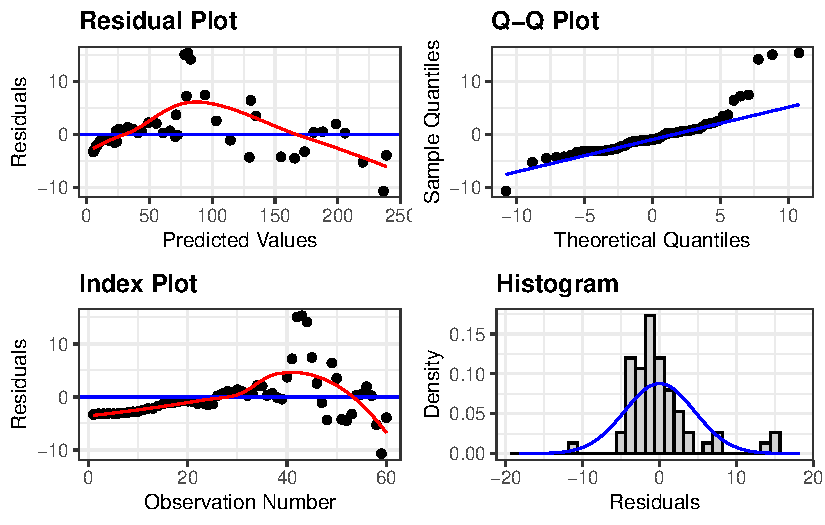
\includegraphics{Spurious-Regressions_files/figure-pdf/unnamed-chunk-3-1.pdf}

This plot shows serious problems, since these residuals display
systematic behavior. They are all negative and small early. To see how
these patterns differ from independent random variables, we provide a
graph of independent random variables with mean 0 and standard error
4.579, matching the estimated regression model standard error. The
Keynesian consumption function is one of the most widely accepted and
estimated regression models. The causal hypothesis is that Income (GDP)
determines Consumption (Con): GDP \(\Rightarrow\) Con. The simplest
regression model which embodies this relationship is: Con = a + b GDP.
Running this regression on the data leads to the following results:

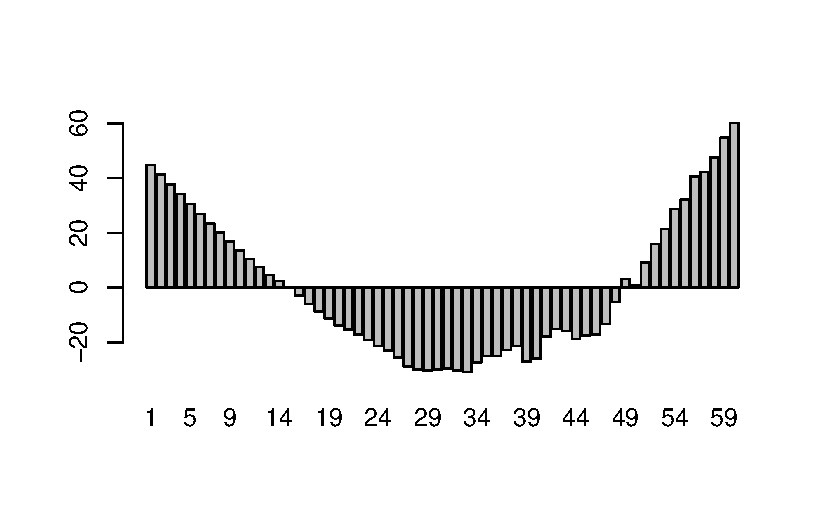
\includegraphics{Spurious-Regressions_files/figure-pdf/unnamed-chunk-4-1.pdf}

Random residuals frequently switch signs. They do not display any
patterns in sequencing. The patterned residuals in the consumption
function prove that the regression is not valid. In such situations,
econometricians typically assume that the problem is due to missing
regressors or wrong functional form. By adding suitable additional
regressors, and modifying the functional form, one can generally ensure
that the residuals appear to satisfy the assumptions made about them.
But, solving the problem of random residuals by this search over
regression models creates a serious problem. This can be explained as
follows. Some of the fits in the data reflect a genuine real-world
relationship. Other patterns are only accidental, and do not reflect any
genuine relationship. The more we search, the more likely we are to end
up with an accidental pattern. The fact that most regression
relationships breakdown very frequently is due to the fact that most of
them are accidental patterns in the data without any counterpart in
reality.

The coefficient of the regressor is supposed to be a measure of the
causal effect. According to the regression above, if SgpGDP goes up by
\$100, then \$49 of it will be spent on consumption. This means that the
enormously high proportion of 51\% of the income will be saved. Since
savings translate to investments, this could account for the dramatic
growth of Singapore over the period in question. However, the patterns
shown in the errors show that we cannot rely on the validity of this
estimate. Vast amounts of experience with estimating this kind of
regression function leads to two major conclusions.

\begin{verbatim}
1.The estimate 0.49 of the causal effect is highly unstable – by adding many
different plausible variables, we can make it change over a great range of
values. Thus, these regressions do not provide accurate estimates of the key
parameter we want to estimate.
2.The best fitting regressions very often make huge forecasting errors, and
therefore are not very useful for policy. 
\end{verbatim}

Even though the regression is not very useful in estimating the size of
the causal effect, at least the high R-squared SEEMS to confirm the
causal effect that SgpGDP =\textgreater{} SdpCon. At least, that was
widely believed before the 1980's: high R-squared means that you have a
good regression equation. It is this issue that we want to examine in
this lecture. That is, we want to clarify how nonsense regressions can
have high R-squared.

\hypertarget{a-spurious-regression-correlation-without-causation}{%
\subsection{A Spurious Regression: Correlation without
Causation}\label{a-spurious-regression-correlation-without-causation}}

First, let us just demonstrate the problem by running a nonsense
regression of SgpCon on SAfGDP -- what is the relationship of Singapore
Consumption with South African GDP. Before running the regression, we
know that it is nonsense -- there should be no relationship, or very
little relationship between these two variables. Here is a graph of the
two series, re-scaled:

A regression of SgpCon on SAfGDP yields: SgpCon = 16.99 + 0.517 SAfGDP:
\(R^2\) is 97\%, and the \(t-stat\) of 40.8 on the coefficient 0.517 is
very high. Based on the p-value of 0.000, we can safely reject the null
hypothesis that the coefficient of SAfGDP is 0. But this is a
nonsensical conclusion, if interpreted causally. It is not even remotely
possible that a 100 Rand increase in South African GDP will increase
consumption in Singapore by 51.7 Singapore Dollars. The central goal of
this lecture is to highlight the dramatic difference between this
regression and the previous one. While the previous equation of SgpCon
on SgpGDP suffers from many defects, it is built on the right
foundations of a causal relationship: SgpGDP =\textgreater{} SgpCon. The
estimated causal coefficient of 0.486 is most likely wrong, because the
residuals show patterns violating the assumptions of the regression
model. But there is a right coefficient, and we can have hope that we
can get to a better estimate by adjusting the equation to fix the flaws
in it. In contrast, there is no causal relationship between SAfGDP and
SgpCon. The estimated coefficient 0.517 of SAfGDP in the second equation
is purely mythical -- it is measuring something which does not exist.
What lesson do we learn from the fact that, despite this difference,
both equations look more or less the same on the surface, with respect
to the statistics produced by the regression package? This is discussed
in the next section.

\hypertarget{the-distinction-between-nominal-and-real-econometrics}{%
\subsection{The Distinction Between Nominal and Real
Econometrics}\label{the-distinction-between-nominal-and-real-econometrics}}

The central problem with conventional econometrics textbooks is the
failure to clarify the difference between correlation and causation. The
world of difference between the first and second equation above exists
because the first equation attempts to estimate a causal coefficient,
while the second provides an estimate of the correlation. Most students
of conventional econometrics are never taught the difference between the
two. To understand the deeper reason for this failure, it is useful to
distinguish between ``nominal'' and ``real'' econometrics. By nominal,
we mean econometrics techniques for which the names of the variables X
and Y are sufficient, and we have no concern with the meaning of these
names in the real world. The vast majority of econometrics taught in
popular textbooks is nominal -- it can be applied to any X and Y. In
contrast, real econometrics is concerned with meaning. It is an aspect
of real econometrics that the consumption function involves regression
of Consumption on GDP and not the other way around. We know that the
causation runs from income to consumption in the real world. ALL causal
relationships are real world relationships which reflect the operation
of real-world mechanisms linking the variables under study. Real
relationships cannot be studied within a nominal framework, and this is
why conventional textbooks fail to come to grips with the problems
created by nonsense regressions. The distinction between the regression
of SgpCon on SgpGDP versus SgpCon on SAfGDP is clear in real
econometrics, but cannot be explained in nominal econometrics. More
generally, conventional regression methods fail to specify the causal
structures governing the variables under study, and hence fail to
differentiate between causation and correlation.

It is useful to clarify the correct interpretation of the coefficient
0.517 of SAfGDP in the second regression. This measures a correlation
that increases in SAfGDP and in SgpCon has happened together
(correlation) in the past. If we observe a 100 Rand increase in SAfGDP,
we could predict a \$51.7 in SgpCon, on the basis of past patterns of
correlation. Because this correlation is not based on any underlying
causal relationship, it could easily break down in the future.
Furthermore, one essential difference between causation and correlation
has to do with INTERVENTIONS. The meaning of the causal relationship X
\(\Rightarrow\) Y is that changes in X will lead to changes in Y. In
contrast, correlations break down under interventions. If we change
SAfGDP, we would not expect to see any change in SgpCon. But we know
this from ``real'' considerations -- we cannot learn this from anything
in the data by themselves.

\hypertarget{the-nominalist-solutions}{%
\subsection{The Nominalist Solutions}\label{the-nominalist-solutions}}

The deeper point is that assessing whether or not a relationship is
causal ALWAYS requires going beyond the names of the variables to the
real-world concepts represented by the variables. This is why nominal
econometrics is unable to distinguish between sensible regressions and
nonsense regressions. This point will be argued and defended in detail
later in the course. At this point, we will simply illustrate one class
of nonsense regressions which have been widely recognized and
acknowledged in the econometrics literature. Decades have been spent
searching for a cure for this problem -- how to distinguish between
sense and nonsense -- but no answers have been found. This is because no
answers can be found within the methodology of nominalist econometrics.

The real solution to the problem of nonsense regressions can only be
found by deeper study of causal structures connecting the variables
under study. This involves stepping outside the boundaries of nominal
econometrics. We will discuss some basics of real econometrics based on
causal path diagrams later in this course. The phenomenon of spurious or
nonensense regression was highlighted by Granger and Newbold in 1980,
the search for solutions has spanned the past few decades. None of these
have been successful. We discuss three main approaches developed for
this problem below.

\hypertarget{missing-variables}{%
\subsection{Missing Variables}\label{missing-variables}}

In the second regression, which regresses SgpCon on SAfGDP, the
regression has a very high R-squared, and the coefficient of South
African GDP is highly significant. This conveys the misleading message
that SAfGDP is an extremely important determinant of SgpCon. The
traditional ``nominalist'' understanding of this problem is that it
arises from missing variables. The equation is giving us the wrong
message, because the central determinant of SgpCon, which is SgpGDP, has
been excluded from the equation. This leads to ``Omitted Variables
Bias''. Failure to put in the correct variables leads to SgpGDP acting
as a proxy for the omitted variable, which is why it has a significant
coefficient. Based on this approach, we can correct the problem by
putting in the missing variable. Accordingly, we run a regression of
SgpCon on both SgpGDP and SAfGDP. We expect that now, the SdgGDP will
come out significant, and the SAfGDP will no longer be significant.
However, the regression result is the following:

\hypertarget{variable-transformation-to-stationarity}{%
\subsection{Variable Transformation to
Stationarity:}\label{variable-transformation-to-stationarity}}

The reason for the failure of trend fit may be due to the reasonable
assumption that the growth rate is stable across time, so that
con\_gr=(SgpCon-lag(SgpCon,1))/lag(SgpCon,1)\emph{100,gdp\_gr=(SgpGDP-lag(SgpGDP,1))/lag(SgpGDP,1)}100,gdp\_gr\_Saf=(SAfGDP-lag(SAfGDP,1))/lag(SAfGDP,1)*100
would be uncorrelated with time. This can be checked by graphing this
variable against time, as follows:

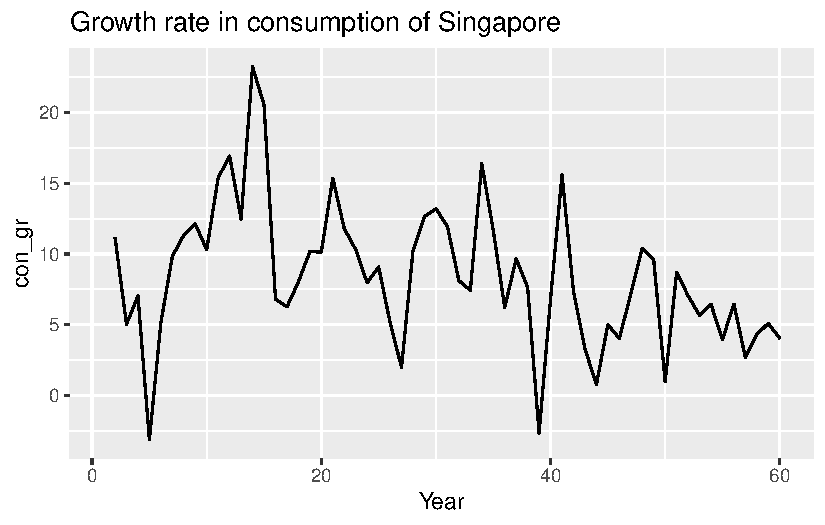
\includegraphics{Spurious-Regressions_files/figure-pdf/unnamed-chunk-5-1.pdf}

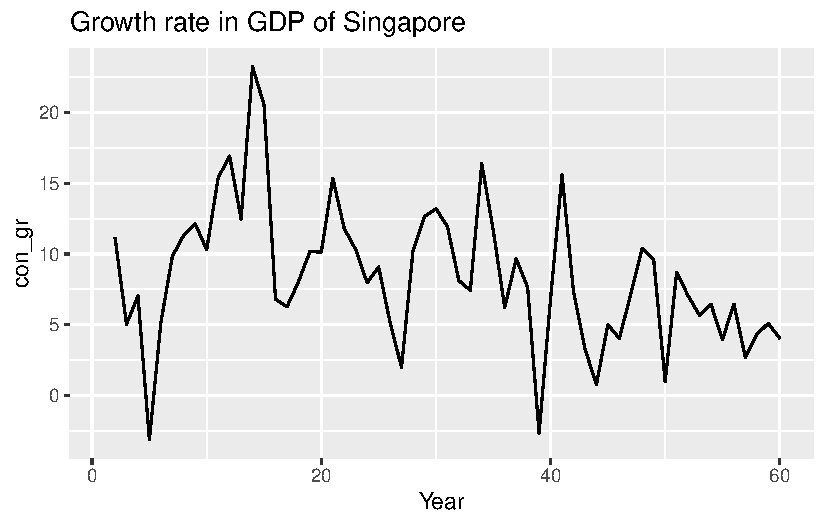
\includegraphics{Spurious-Regressions_files/figure-pdf/unnamed-chunk-5-2.pdf}

 
  \providecommand{\huxb}[2]{\arrayrulecolor[RGB]{#1}\global\arrayrulewidth=#2pt}
  \providecommand{\huxvb}[2]{\color[RGB]{#1}\vrule width #2pt}
  \providecommand{\huxtpad}[1]{\rule{0pt}{#1}}
  \providecommand{\huxbpad}[1]{\rule[-#1]{0pt}{#1}}

\begin{table}[ht]
\begin{centerbox}
\begin{threeparttable}
 
\setlength{\tabcolsep}{0pt}
\begin{tabular}{l l}


\hhline{>{\huxb{0, 0, 0}{0.8}}->{\huxb{0, 0, 0}{0.8}}-}
\arrayrulecolor{black}

\multicolumn{1}{!{\huxvb{0, 0, 0}{0}}c!{\huxvb{0, 0, 0}{0}}}{\huxtpad{6pt + 1em}\centering \hspace{6pt}  \hspace{6pt}\huxbpad{6pt}} &
\multicolumn{1}{c!{\huxvb{0, 0, 0}{0}}}{\huxtpad{6pt + 1em}\centering \hspace{6pt} (1) \hspace{6pt}\huxbpad{6pt}} \tabularnewline[-0.5pt]


\hhline{>{\huxb{255, 255, 255}{0.4}}->{\huxb{0, 0, 0}{0.4}}-}
\arrayrulecolor{black}

\multicolumn{1}{!{\huxvb{0, 0, 0}{0}}l!{\huxvb{0, 0, 0}{0}}}{\huxtpad{6pt + 1em}\raggedright \hspace{6pt} (Intercept) \hspace{6pt}\huxbpad{6pt}} &
\multicolumn{1}{r!{\huxvb{0, 0, 0}{0}}}{\huxtpad{6pt + 1em}\raggedleft \hspace{6pt} 2.162 **\hphantom{0} \hspace{6pt}\huxbpad{6pt}} \tabularnewline[-0.5pt]


\hhline{}
\arrayrulecolor{black}

\multicolumn{1}{!{\huxvb{0, 0, 0}{0}}l!{\huxvb{0, 0, 0}{0}}}{\huxtpad{6pt + 1em}\raggedright \hspace{6pt}  \hspace{6pt}\huxbpad{6pt}} &
\multicolumn{1}{r!{\huxvb{0, 0, 0}{0}}}{\huxtpad{6pt + 1em}\raggedleft \hspace{6pt} (0.661)\hphantom{0}\hphantom{0}\hphantom{0} \hspace{6pt}\huxbpad{6pt}} \tabularnewline[-0.5pt]


\hhline{}
\arrayrulecolor{black}

\multicolumn{1}{!{\huxvb{0, 0, 0}{0}}l!{\huxvb{0, 0, 0}{0}}}{\huxtpad{6pt + 1em}\raggedright \hspace{6pt} gdp\_gr \hspace{6pt}\huxbpad{6pt}} &
\multicolumn{1}{r!{\huxvb{0, 0, 0}{0}}}{\huxtpad{6pt + 1em}\raggedleft \hspace{6pt} 0.635 *** \hspace{6pt}\huxbpad{6pt}} \tabularnewline[-0.5pt]


\hhline{}
\arrayrulecolor{black}

\multicolumn{1}{!{\huxvb{0, 0, 0}{0}}l!{\huxvb{0, 0, 0}{0}}}{\huxtpad{6pt + 1em}\raggedright \hspace{6pt}  \hspace{6pt}\huxbpad{6pt}} &
\multicolumn{1}{r!{\huxvb{0, 0, 0}{0}}}{\huxtpad{6pt + 1em}\raggedleft \hspace{6pt} (0.056)\hphantom{0}\hphantom{0}\hphantom{0} \hspace{6pt}\huxbpad{6pt}} \tabularnewline[-0.5pt]


\hhline{>{\huxb{255, 255, 255}{0.4}}->{\huxb{0, 0, 0}{0.4}}-}
\arrayrulecolor{black}

\multicolumn{1}{!{\huxvb{0, 0, 0}{0}}l!{\huxvb{0, 0, 0}{0}}}{\huxtpad{6pt + 1em}\raggedright \hspace{6pt} N \hspace{6pt}\huxbpad{6pt}} &
\multicolumn{1}{r!{\huxvb{0, 0, 0}{0}}}{\huxtpad{6pt + 1em}\raggedleft \hspace{6pt} 59\hphantom{0}\hphantom{0}\hphantom{0}\hphantom{0}\hphantom{0}\hphantom{0}\hphantom{0}\hphantom{0} \hspace{6pt}\huxbpad{6pt}} \tabularnewline[-0.5pt]


\hhline{}
\arrayrulecolor{black}

\multicolumn{1}{!{\huxvb{0, 0, 0}{0}}l!{\huxvb{0, 0, 0}{0}}}{\huxtpad{6pt + 1em}\raggedright \hspace{6pt} R2 \hspace{6pt}\huxbpad{6pt}} &
\multicolumn{1}{r!{\huxvb{0, 0, 0}{0}}}{\huxtpad{6pt + 1em}\raggedleft \hspace{6pt} 0.694\hphantom{0}\hphantom{0}\hphantom{0}\hphantom{0} \hspace{6pt}\huxbpad{6pt}} \tabularnewline[-0.5pt]


\hhline{}
\arrayrulecolor{black}

\multicolumn{1}{!{\huxvb{0, 0, 0}{0}}l!{\huxvb{0, 0, 0}{0}}}{\huxtpad{6pt + 1em}\raggedright \hspace{6pt} logLik \hspace{6pt}\huxbpad{6pt}} &
\multicolumn{1}{r!{\huxvb{0, 0, 0}{0}}}{\huxtpad{6pt + 1em}\raggedleft \hspace{6pt} -143.053\hphantom{0}\hphantom{0}\hphantom{0}\hphantom{0} \hspace{6pt}\huxbpad{6pt}} \tabularnewline[-0.5pt]


\hhline{}
\arrayrulecolor{black}

\multicolumn{1}{!{\huxvb{0, 0, 0}{0}}l!{\huxvb{0, 0, 0}{0}}}{\huxtpad{6pt + 1em}\raggedright \hspace{6pt} AIC \hspace{6pt}\huxbpad{6pt}} &
\multicolumn{1}{r!{\huxvb{0, 0, 0}{0}}}{\huxtpad{6pt + 1em}\raggedleft \hspace{6pt} 292.105\hphantom{0}\hphantom{0}\hphantom{0}\hphantom{0} \hspace{6pt}\huxbpad{6pt}} \tabularnewline[-0.5pt]


\hhline{>{\huxb{0, 0, 0}{0.8}}->{\huxb{0, 0, 0}{0.8}}-}
\arrayrulecolor{black}

\multicolumn{2}{!{\huxvb{0, 0, 0}{0}}l!{\huxvb{0, 0, 0}{0}}}{\huxtpad{6pt + 1em}\raggedright \hspace{6pt}  *** p $<$ 0.001;  ** p $<$ 0.01;  * p $<$ 0.05. \hspace{6pt}\huxbpad{6pt}} \tabularnewline[-0.5pt]


\hhline{}
\arrayrulecolor{black}
\end{tabular}
\end{threeparttable}\par\end{centerbox}

\end{table}
 

This variable is also uncorrelated with time, at least visually. The
variable transformation of taking growth rates has removed the common
time trend from both variables. Now it should be possible to run a
regression of Consumption on Income which does not suffer from the
spurious correlation between the two variables created by the common
trend. Unfortunately, this strategy also fails to differentiate between
genuine and spurious regressions as we will see. First, let us look at
the genuine causal regression of Gr\_SgpC on Gr\_SgfG: Gr\_SdpC = 0.009
+ 0.634 Gr\_SgpG \(R^2\) is now 69\%. It has gone down because we have
removed the correlation due to the common factor of time-trend, but it
is still very high. The regression provides a good fit. Also, for the
first time, the residuals from this regression look random:

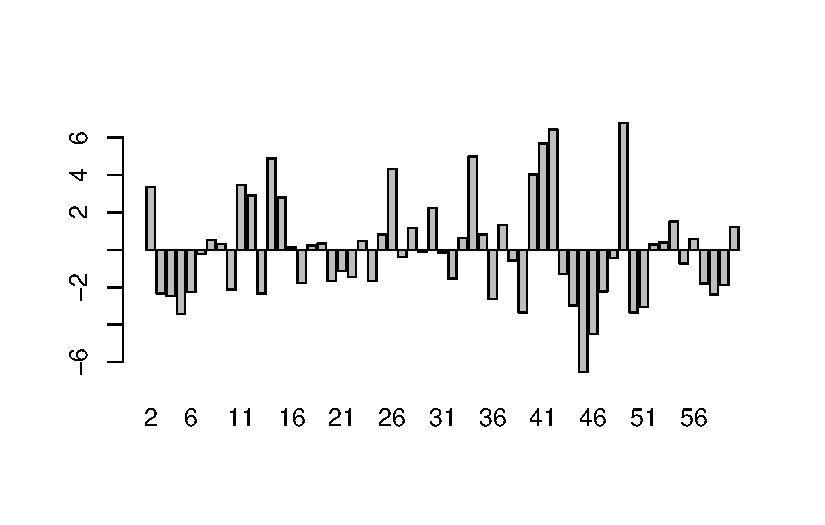
\includegraphics{Spurious-Regressions_files/figure-pdf/unnamed-chunk-6-1.pdf}

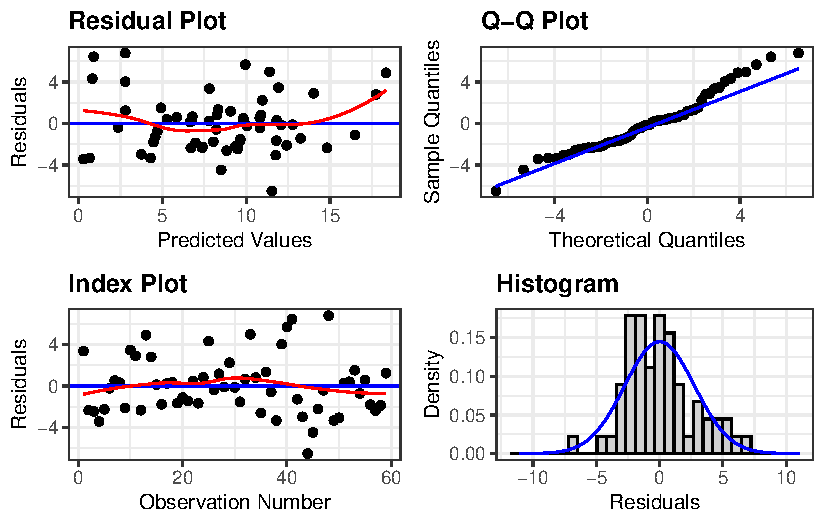
\includegraphics{Spurious-Regressions_files/figure-pdf/unnamed-chunk-6-2.pdf}

This transformation from levels to growth rates has substantially
improved the regression results. There is now some hope that the
coefficient 0.634 might be a correct measure of a causal effect, if
other aspects of the specification are also correct.

However, our main concern is to see if this transformation can
distinguish between genuine causal relationships and spurious ones. For
this purpose, we run the regression of the growth rate of SgpCon on the
growth rate of SAfGDP. This yields the following results:

 
  \providecommand{\huxb}[2]{\arrayrulecolor[RGB]{#1}\global\arrayrulewidth=#2pt}
  \providecommand{\huxvb}[2]{\color[RGB]{#1}\vrule width #2pt}
  \providecommand{\huxtpad}[1]{\rule{0pt}{#1}}
  \providecommand{\huxbpad}[1]{\rule[-#1]{0pt}{#1}}

\begin{table}[ht]
\begin{centerbox}
\begin{threeparttable}
 
\setlength{\tabcolsep}{0pt}
\begin{tabular}{l l}


\hhline{>{\huxb{0, 0, 0}{0.8}}->{\huxb{0, 0, 0}{0.8}}-}
\arrayrulecolor{black}

\multicolumn{1}{!{\huxvb{0, 0, 0}{0}}c!{\huxvb{0, 0, 0}{0}}}{\huxtpad{6pt + 1em}\centering \hspace{6pt}  \hspace{6pt}\huxbpad{6pt}} &
\multicolumn{1}{c!{\huxvb{0, 0, 0}{0}}}{\huxtpad{6pt + 1em}\centering \hspace{6pt} (1) \hspace{6pt}\huxbpad{6pt}} \tabularnewline[-0.5pt]


\hhline{>{\huxb{255, 255, 255}{0.4}}->{\huxb{0, 0, 0}{0.4}}-}
\arrayrulecolor{black}

\multicolumn{1}{!{\huxvb{0, 0, 0}{0}}l!{\huxvb{0, 0, 0}{0}}}{\huxtpad{6pt + 1em}\raggedright \hspace{6pt} (Intercept) \hspace{6pt}\huxbpad{6pt}} &
\multicolumn{1}{r!{\huxvb{0, 0, 0}{0}}}{\huxtpad{6pt + 1em}\raggedleft \hspace{6pt} 1.822\hphantom{0}\hphantom{0}\hphantom{0}\hphantom{0} \hspace{6pt}\huxbpad{6pt}} \tabularnewline[-0.5pt]


\hhline{}
\arrayrulecolor{black}

\multicolumn{1}{!{\huxvb{0, 0, 0}{0}}l!{\huxvb{0, 0, 0}{0}}}{\huxtpad{6pt + 1em}\raggedright \hspace{6pt}  \hspace{6pt}\huxbpad{6pt}} &
\multicolumn{1}{r!{\huxvb{0, 0, 0}{0}}}{\huxtpad{6pt + 1em}\raggedleft \hspace{6pt} (1.407)\hphantom{0}\hphantom{0}\hphantom{0} \hspace{6pt}\huxbpad{6pt}} \tabularnewline[-0.5pt]


\hhline{}
\arrayrulecolor{black}

\multicolumn{1}{!{\huxvb{0, 0, 0}{0}}l!{\huxvb{0, 0, 0}{0}}}{\huxtpad{6pt + 1em}\raggedright \hspace{6pt} gdp\_gr\_Saf \hspace{6pt}\huxbpad{6pt}} &
\multicolumn{1}{r!{\huxvb{0, 0, 0}{0}}}{\huxtpad{6pt + 1em}\raggedleft \hspace{6pt} 0.539 *** \hspace{6pt}\huxbpad{6pt}} \tabularnewline[-0.5pt]


\hhline{}
\arrayrulecolor{black}

\multicolumn{1}{!{\huxvb{0, 0, 0}{0}}l!{\huxvb{0, 0, 0}{0}}}{\huxtpad{6pt + 1em}\raggedright \hspace{6pt}  \hspace{6pt}\huxbpad{6pt}} &
\multicolumn{1}{r!{\huxvb{0, 0, 0}{0}}}{\huxtpad{6pt + 1em}\raggedleft \hspace{6pt} (0.106)\hphantom{0}\hphantom{0}\hphantom{0} \hspace{6pt}\huxbpad{6pt}} \tabularnewline[-0.5pt]


\hhline{>{\huxb{255, 255, 255}{0.4}}->{\huxb{0, 0, 0}{0.4}}-}
\arrayrulecolor{black}

\multicolumn{1}{!{\huxvb{0, 0, 0}{0}}l!{\huxvb{0, 0, 0}{0}}}{\huxtpad{6pt + 1em}\raggedright \hspace{6pt} N \hspace{6pt}\huxbpad{6pt}} &
\multicolumn{1}{r!{\huxvb{0, 0, 0}{0}}}{\huxtpad{6pt + 1em}\raggedleft \hspace{6pt} 59\hphantom{0}\hphantom{0}\hphantom{0}\hphantom{0}\hphantom{0}\hphantom{0}\hphantom{0}\hphantom{0} \hspace{6pt}\huxbpad{6pt}} \tabularnewline[-0.5pt]


\hhline{}
\arrayrulecolor{black}

\multicolumn{1}{!{\huxvb{0, 0, 0}{0}}l!{\huxvb{0, 0, 0}{0}}}{\huxtpad{6pt + 1em}\raggedright \hspace{6pt} R2 \hspace{6pt}\huxbpad{6pt}} &
\multicolumn{1}{r!{\huxvb{0, 0, 0}{0}}}{\huxtpad{6pt + 1em}\raggedleft \hspace{6pt} 0.313\hphantom{0}\hphantom{0}\hphantom{0}\hphantom{0} \hspace{6pt}\huxbpad{6pt}} \tabularnewline[-0.5pt]


\hhline{}
\arrayrulecolor{black}

\multicolumn{1}{!{\huxvb{0, 0, 0}{0}}l!{\huxvb{0, 0, 0}{0}}}{\huxtpad{6pt + 1em}\raggedright \hspace{6pt} logLik \hspace{6pt}\huxbpad{6pt}} &
\multicolumn{1}{r!{\huxvb{0, 0, 0}{0}}}{\huxtpad{6pt + 1em}\raggedleft \hspace{6pt} -166.857\hphantom{0}\hphantom{0}\hphantom{0}\hphantom{0} \hspace{6pt}\huxbpad{6pt}} \tabularnewline[-0.5pt]


\hhline{}
\arrayrulecolor{black}

\multicolumn{1}{!{\huxvb{0, 0, 0}{0}}l!{\huxvb{0, 0, 0}{0}}}{\huxtpad{6pt + 1em}\raggedright \hspace{6pt} AIC \hspace{6pt}\huxbpad{6pt}} &
\multicolumn{1}{r!{\huxvb{0, 0, 0}{0}}}{\huxtpad{6pt + 1em}\raggedleft \hspace{6pt} 339.714\hphantom{0}\hphantom{0}\hphantom{0}\hphantom{0} \hspace{6pt}\huxbpad{6pt}} \tabularnewline[-0.5pt]


\hhline{>{\huxb{0, 0, 0}{0.8}}->{\huxb{0, 0, 0}{0.8}}-}
\arrayrulecolor{black}

\multicolumn{2}{!{\huxvb{0, 0, 0}{0}}l!{\huxvb{0, 0, 0}{0}}}{\huxtpad{6pt + 1em}\raggedright \hspace{6pt}  *** p $<$ 0.001;  ** p $<$ 0.01;  * p $<$ 0.05. \hspace{6pt}\huxbpad{6pt}} \tabularnewline[-0.5pt]


\hhline{}
\arrayrulecolor{black}
\end{tabular}
\end{threeparttable}\par\end{centerbox}

\end{table}
 

\(Predicted GrSgpC = 0.006484 + 0.566 GrSAfG\)

This regression also shows that growth rates of South African GDP are
highly significant in explaining growth rates of Singaporean
Consumption. The regression residuals look random, and support the
validity of this regression:

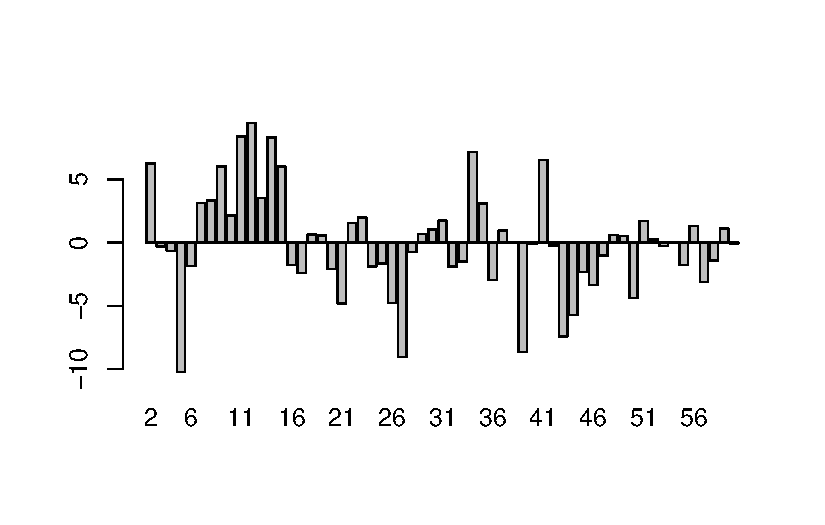
\includegraphics{Spurious-Regressions_files/figure-pdf/unnamed-chunk-8-1.pdf}

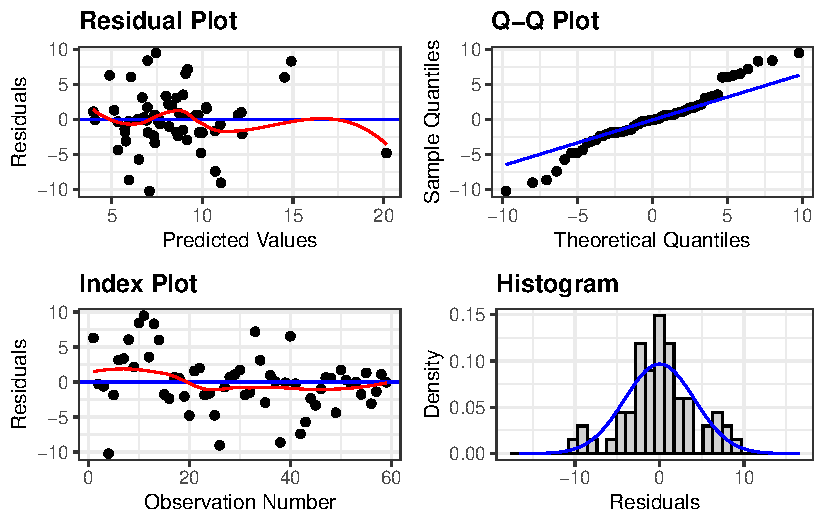
\includegraphics{Spurious-Regressions_files/figure-pdf/unnamed-chunk-8-2.pdf}

According to conventional econometrics, the causal regression of growth
rates of SgpGDP on growth rates of SgpCon allows us to conclude that
63\% of changes in Gr\_SgpGDP are transmitted to Gr\_SgpCon. But, by
exactly the same reasoning, we can use the spurious regression of
Gr\_SgpCon on Gr\_SAfGDP to conclude that 56.6\% of changes in the
growth rate of the South African economy are transmitted to growth rates
of Singaporean consumption. The first measurement has some chance being
correct, while the second statement is ridiculous.

In this particular case, the missing variables strategy can solve the
problem. If we think that the source of the problem in this last
equation is that the primary determinant of SgpCon is missing from the
equation, we can fix the problem by adding this variable. When we do so,
we get the following equation: Gr\_SgpC = 0.004 + 0.163 Gr\_SAfG + 0.569
Gr\_SgpG

 
  \providecommand{\huxb}[2]{\arrayrulecolor[RGB]{#1}\global\arrayrulewidth=#2pt}
  \providecommand{\huxvb}[2]{\color[RGB]{#1}\vrule width #2pt}
  \providecommand{\huxtpad}[1]{\rule{0pt}{#1}}
  \providecommand{\huxbpad}[1]{\rule[-#1]{0pt}{#1}}

\begin{table}[ht]
\begin{centerbox}
\begin{threeparttable}
 
\setlength{\tabcolsep}{0pt}
\begin{tabular}{l l}


\hhline{>{\huxb{0, 0, 0}{0.8}}->{\huxb{0, 0, 0}{0.8}}-}
\arrayrulecolor{black}

\multicolumn{1}{!{\huxvb{0, 0, 0}{0}}c!{\huxvb{0, 0, 0}{0}}}{\huxtpad{6pt + 1em}\centering \hspace{6pt}  \hspace{6pt}\huxbpad{6pt}} &
\multicolumn{1}{c!{\huxvb{0, 0, 0}{0}}}{\huxtpad{6pt + 1em}\centering \hspace{6pt} (1) \hspace{6pt}\huxbpad{6pt}} \tabularnewline[-0.5pt]


\hhline{>{\huxb{255, 255, 255}{0.4}}->{\huxb{0, 0, 0}{0.4}}-}
\arrayrulecolor{black}

\multicolumn{1}{!{\huxvb{0, 0, 0}{0}}l!{\huxvb{0, 0, 0}{0}}}{\huxtpad{6pt + 1em}\raggedright \hspace{6pt} (Intercept) \hspace{6pt}\huxbpad{6pt}} &
\multicolumn{1}{r!{\huxvb{0, 0, 0}{0}}}{\huxtpad{6pt + 1em}\raggedleft \hspace{6pt} 1.032\hphantom{0}\hphantom{0}\hphantom{0}\hphantom{0} \hspace{6pt}\huxbpad{6pt}} \tabularnewline[-0.5pt]


\hhline{}
\arrayrulecolor{black}

\multicolumn{1}{!{\huxvb{0, 0, 0}{0}}l!{\huxvb{0, 0, 0}{0}}}{\huxtpad{6pt + 1em}\raggedright \hspace{6pt}  \hspace{6pt}\huxbpad{6pt}} &
\multicolumn{1}{r!{\huxvb{0, 0, 0}{0}}}{\huxtpad{6pt + 1em}\raggedleft \hspace{6pt} (0.929)\hphantom{0}\hphantom{0}\hphantom{0} \hspace{6pt}\huxbpad{6pt}} \tabularnewline[-0.5pt]


\hhline{}
\arrayrulecolor{black}

\multicolumn{1}{!{\huxvb{0, 0, 0}{0}}l!{\huxvb{0, 0, 0}{0}}}{\huxtpad{6pt + 1em}\raggedright \hspace{6pt} gdp\_gr\_Saf \hspace{6pt}\huxbpad{6pt}} &
\multicolumn{1}{r!{\huxvb{0, 0, 0}{0}}}{\huxtpad{6pt + 1em}\raggedleft \hspace{6pt} 0.141\hphantom{0}\hphantom{0}\hphantom{0}\hphantom{0} \hspace{6pt}\huxbpad{6pt}} \tabularnewline[-0.5pt]


\hhline{}
\arrayrulecolor{black}

\multicolumn{1}{!{\huxvb{0, 0, 0}{0}}l!{\huxvb{0, 0, 0}{0}}}{\huxtpad{6pt + 1em}\raggedright \hspace{6pt}  \hspace{6pt}\huxbpad{6pt}} &
\multicolumn{1}{r!{\huxvb{0, 0, 0}{0}}}{\huxtpad{6pt + 1em}\raggedleft \hspace{6pt} (0.083)\hphantom{0}\hphantom{0}\hphantom{0} \hspace{6pt}\huxbpad{6pt}} \tabularnewline[-0.5pt]


\hhline{}
\arrayrulecolor{black}

\multicolumn{1}{!{\huxvb{0, 0, 0}{0}}l!{\huxvb{0, 0, 0}{0}}}{\huxtpad{6pt + 1em}\raggedright \hspace{6pt} gdp\_gr \hspace{6pt}\huxbpad{6pt}} &
\multicolumn{1}{r!{\huxvb{0, 0, 0}{0}}}{\huxtpad{6pt + 1em}\raggedleft \hspace{6pt} 0.573 *** \hspace{6pt}\huxbpad{6pt}} \tabularnewline[-0.5pt]


\hhline{}
\arrayrulecolor{black}

\multicolumn{1}{!{\huxvb{0, 0, 0}{0}}l!{\huxvb{0, 0, 0}{0}}}{\huxtpad{6pt + 1em}\raggedright \hspace{6pt}  \hspace{6pt}\huxbpad{6pt}} &
\multicolumn{1}{r!{\huxvb{0, 0, 0}{0}}}{\huxtpad{6pt + 1em}\raggedleft \hspace{6pt} (0.066)\hphantom{0}\hphantom{0}\hphantom{0} \hspace{6pt}\huxbpad{6pt}} \tabularnewline[-0.5pt]


\hhline{>{\huxb{255, 255, 255}{0.4}}->{\huxb{0, 0, 0}{0.4}}-}
\arrayrulecolor{black}

\multicolumn{1}{!{\huxvb{0, 0, 0}{0}}l!{\huxvb{0, 0, 0}{0}}}{\huxtpad{6pt + 1em}\raggedright \hspace{6pt} N \hspace{6pt}\huxbpad{6pt}} &
\multicolumn{1}{r!{\huxvb{0, 0, 0}{0}}}{\huxtpad{6pt + 1em}\raggedleft \hspace{6pt} 59\hphantom{0}\hphantom{0}\hphantom{0}\hphantom{0}\hphantom{0}\hphantom{0}\hphantom{0}\hphantom{0} \hspace{6pt}\huxbpad{6pt}} \tabularnewline[-0.5pt]


\hhline{}
\arrayrulecolor{black}

\multicolumn{1}{!{\huxvb{0, 0, 0}{0}}l!{\huxvb{0, 0, 0}{0}}}{\huxtpad{6pt + 1em}\raggedright \hspace{6pt} R2 \hspace{6pt}\huxbpad{6pt}} &
\multicolumn{1}{r!{\huxvb{0, 0, 0}{0}}}{\huxtpad{6pt + 1em}\raggedleft \hspace{6pt} 0.709\hphantom{0}\hphantom{0}\hphantom{0}\hphantom{0} \hspace{6pt}\huxbpad{6pt}} \tabularnewline[-0.5pt]


\hhline{}
\arrayrulecolor{black}

\multicolumn{1}{!{\huxvb{0, 0, 0}{0}}l!{\huxvb{0, 0, 0}{0}}}{\huxtpad{6pt + 1em}\raggedright \hspace{6pt} logLik \hspace{6pt}\huxbpad{6pt}} &
\multicolumn{1}{r!{\huxvb{0, 0, 0}{0}}}{\huxtpad{6pt + 1em}\raggedleft \hspace{6pt} -141.561\hphantom{0}\hphantom{0}\hphantom{0}\hphantom{0} \hspace{6pt}\huxbpad{6pt}} \tabularnewline[-0.5pt]


\hhline{}
\arrayrulecolor{black}

\multicolumn{1}{!{\huxvb{0, 0, 0}{0}}l!{\huxvb{0, 0, 0}{0}}}{\huxtpad{6pt + 1em}\raggedright \hspace{6pt} AIC \hspace{6pt}\huxbpad{6pt}} &
\multicolumn{1}{r!{\huxvb{0, 0, 0}{0}}}{\huxtpad{6pt + 1em}\raggedleft \hspace{6pt} 291.121\hphantom{0}\hphantom{0}\hphantom{0}\hphantom{0} \hspace{6pt}\huxbpad{6pt}} \tabularnewline[-0.5pt]


\hhline{>{\huxb{0, 0, 0}{0.8}}->{\huxb{0, 0, 0}{0.8}}-}
\arrayrulecolor{black}

\multicolumn{2}{!{\huxvb{0, 0, 0}{0}}l!{\huxvb{0, 0, 0}{0}}}{\huxtpad{6pt + 1em}\raggedright \hspace{6pt}  *** p $<$ 0.001;  ** p $<$ 0.01;  * p $<$ 0.05. \hspace{6pt}\huxbpad{6pt}} \tabularnewline[-0.5pt]


\hhline{}
\arrayrulecolor{black}
\end{tabular}
\end{threeparttable}\par\end{centerbox}

\end{table}
 

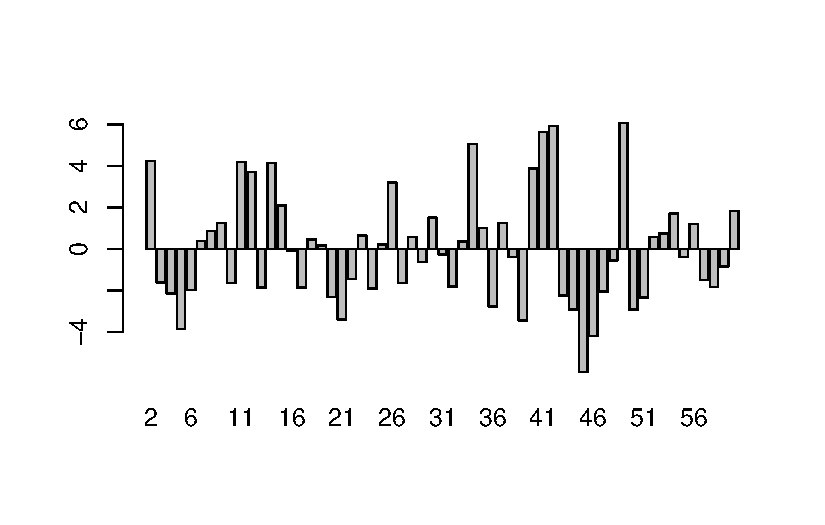
\includegraphics{Spurious-Regressions_files/figure-pdf/unnamed-chunk-10-1.pdf}

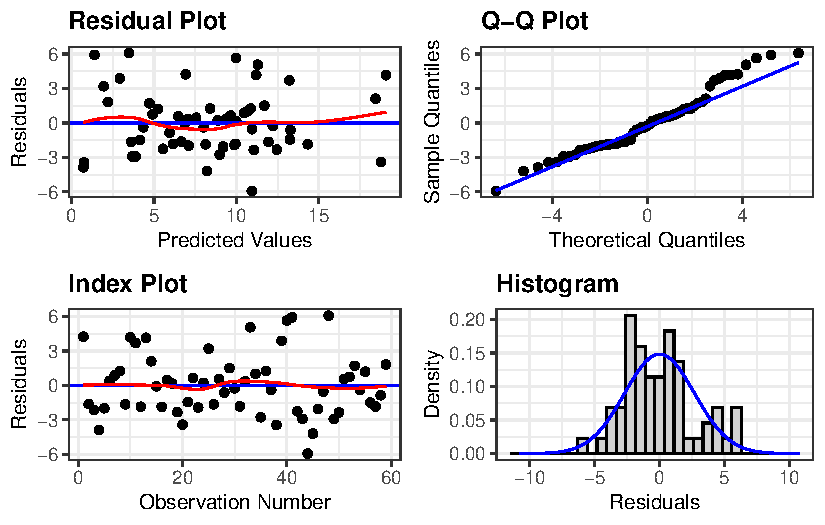
\includegraphics{Spurious-Regressions_files/figure-pdf/unnamed-chunk-10-2.pdf}

Putting in growth rates of both Singapore and South Africa leads to the
right result: Singapore GDP is a highly significant determinant, while
South African GDP is not significant at the 95\% level. Nominal
econometrics consists of this kind of exercise, where we try one
equation after another in order to get a match to our a priori ideas
about the size and strength of the causal effects. This is quite the
opposite of what students are taught about this methodology. It is not
that we allow the data to tell us about the causal structures in the
world. Rather, we know these structures in advance, and try many
different formulations until we get one which matches our
preconceptions.

\hypertarget{concluding-remarks}{%
\subsection{Concluding Remarks}\label{concluding-remarks}}

\emph{Econometricians} have been working on finding methods to
discriminate between nonsense and sensible regressions for decades,
without success. We have discussed three strategies for doing so in this
lecture. All three lead to failure, although the third one can be
salvaged. Currently, it is the third strategy which dominates the scene.
However, it also suffers from failures in many different cases. The
reason for this failure is that solutions to causal problems cannot be
found in nominal econometrics. Without having a good grasp of the causal
structures which relate the regressors to the dependent variables, it is
not possible to estimate causal effects.

POSTSCRIPT: Regressions for the lecture above were done using the
RegressIt package for EXCEL -- available
from:\href{https://regressit.com/}{data} . The WDI Data Set for
Singapore and South Africa, Consumption and GDP, is available from
\href{https://onedrive.live.com/view.aspx?resid=F5F6A4108BE920A5!46844\&ithint=file\%2cxlsx\&authkey=!AA5r8iTFTqYaIfU}{Singapore
Data}



\end{document}
